\documentclass[11pt,a4paper]{article}
\usepackage[margin=2.2cm]{geometry}
\usepackage{amsmath,amssymb}
\usepackage{booktabs}
\usepackage{graphicx}
\usepackage{xcolor}
\usepackage{caption}
\usepackage[colorlinks=true,linkcolor=black,urlcolor=blue]{hyperref}
\usepackage{enumitem}
\setlist{nosep,leftmargin=1.3em}
\captionsetup{font=small,labelfont=bf}
\renewcommand{\arraystretch}{1.15}
\setlength{\parskip}{0.45em}
\setlength{\parindent}{0pt}

\title{\vspace{-1.4cm}\textbf{LoRA Rank and Domain Adaptation of Stable Diffusion~1.5\\to Cityscapes}\\[0.3em]\large Progress report}
\author{Narmeen Sabah Siddiqui}
\date{22 September 2026}

\begin{document}
\maketitle
\vspace{-0.8em}

\section*{1\quad Objective}

Measure how LoRA rank affects domain adaptation of Stable Diffusion~1.5 to the
Cityscapes visual domain, evaluated with FID, KID, CLIPScore, BLIP image--text
matching and LPIPS diversity against real Cityscapes imagery.

Ranks under study: $\{8, 16, 32, 64, 128\}$, plus a frozen SD~1.5 baseline and
the real images as reference.

\section*{2\quad Dataset and preprocessing}

\begin{table}[h]\centering\small
\begin{tabular}{lrrr}
\toprule
Split & Source images & Cities & Cropped \\
\midrule
\texttt{train}       & 2\,975  & 18 & 2\,975 \\
\texttt{val}         & 500     & 3  & 500 \\
\texttt{test}        & 1\,525  & 6  & 1\,525 \\
\texttt{train\_extra}& 19\,997 & 23 & 19\,995 \\
\midrule
\textbf{Total}       & \textbf{24\,997} & \textbf{50} & \textbf{24\,995} \\
\bottomrule
\end{tabular}
\caption{Cityscapes \texttt{leftImg8bit}. Two images were rejected (see below).}
\end{table}

\textbf{Cropping.} Every source frame is $2048\times1024$. We take the central
$1024\times1024$ square with PIL crop box $(512,0,1536,1024)$ --- a crop, not a
resize, so no aspect distortion. All 24\,995 outputs were verified to be exactly
$1024\times1024$.

\textbf{Rejections.} A validity guard skipped zero-byte files, undecodable
files, and frames whose mean pixel value was $<5$ (all-black). Beyond the one
known corrupt frame (\texttt{troisdorf\_000000\_000073}, deleted previously), the
guard caught \textbf{two further all-black frames}:
\texttt{heidelberg\_000000\_000293} (mean 4.97) and
\texttt{oberhausen\_000000\_000899} (mean 4.58). Hence $24\,997 - 2 = 24\,995$.

\textbf{Data split policy.} We do \emph{not} hold out a test split. Section~4
explains why this does not risk memorisation, and why holding out would cost
more in metric precision than it buys in purity.

\section*{3\quad Captioning}

Florence-2-large with task \texttt{<DETAILED\_CAPTION>}; 3 beams;
\texttt{max\_new\_tokens}~$=1024$; greedy decoding. Leading
boilerplate (``The image shows/depicts/features'', ``This image shows'') was
stripped and the first letter re-capitalised.

\begin{table}[h]\centering\small
\begin{tabular}{lr}
\toprule
Captions generated & 24\,995 \\
Distinct captions & 18\,595 \quad(74.4\%) \\
Captions used more than once & 1\,819, covering 8\,219 images \\
Largest duplicate group & 105 images share one caption \\
Length (words) & mean 35.0, median 35, range 14--75 \\
Length (CLIP tokens) & mean 43.3, median 43, p99 66, max 92 \\
Exceeding CLIP's 77-token limit & 15 images (0.06\%) \\
\bottomrule
\end{tabular}
\caption{Caption statistics. Runtime 3\,h\,52\,m on one A100.}
\end{table}

\section*{4\quad Experimental design: prompts, seeds and pairing}

This section answers the question of what is held constant across conditions.

\textbf{Index convention.} The caption file \texttt{metadata.jsonl} is ordered
\texttt{test} $\rightarrow$ \texttt{train} $\rightarrow$ \texttt{train\_extra}
$\rightarrow$ \texttt{val}, with cities and filenames sorted. Its \emph{line
number is the image index}:

\begin{center}\small
\begin{tabular}{lr}
\toprule
\texttt{test} & indices 0--1\,524 \quad(1\,525) \\
\texttt{train} & indices 1\,525--4\,499 \quad(2\,975) \\
\texttt{train\_extra} & indices 4\,500--24\,494 \quad(19\,995) \\
\texttt{val} & indices 24\,495--24\,994 \quad(500) \\
\bottomrule
\end{tabular}
\end{center}

\textbf{Are the prompts the same across ranks and checkpoints? Yes --- exactly.}
Image $i$ in \emph{every} generated set is produced from caption line $i$ with
generator seed $i$:
\[
\texttt{generator} = \texttt{torch.Generator("cuda").manual\_seed}(i).
\]
Consequently prompt 4\,217 receives the identical caption \emph{and} the
identical initial latent noise under the frozen model, under every rank, and
under every checkpoint. The only variable that differs between conditions is the
adapter. This makes the comparison \textbf{paired}: per-image metrics
(CLIP, BLIP) admit a paired test, and set-level metrics (FID, KID) are not
contaminated by prompt-sampling variance.

We verified on disk that for index 4\,714 the frozen and rank-8 mappings agree
with caption line 4\,714, and that all 50 checkpoint directories contain an
\emph{identical} index set.

\textbf{Checkpoint-sweep sample.} Scoring all 24\,995 prompts for every
rank$\times$checkpoint cell is infeasible, so each cell uses a strided
subsample, \texttt{stride}~$=50$: indices $0, 50, 100, \dots, 24\,950$, i.e.\
\textbf{500 images per cell}. A contiguous head would have been all Berlin
test images; the stride instead reproduces the corpus composition almost exactly:

\begin{center}\small
\begin{tabular}{lrr}
\toprule
Split & In 500-sample & Full corpus \\
\midrule
\texttt{test} & 31 \ (6.2\%) & 6.1\% \\
\texttt{train} & 59 \ (11.8\%) & 11.9\% \\
\texttt{train\_extra} & 400 \ (80.0\%) & 80.0\% \\
\texttt{val} & 10 \ (2.0\%) & 2.0\% \\
\bottomrule
\end{tabular}
\end{center}

50 cities are represented. The same 500 indices are used in all 50 cells and for
the frozen baseline, so every number in Section~7 is computed on identical inputs.

\textbf{Why no held-out split.} Caption duplication makes
memorisation-via-caption structurally implausible: a caption does not identify an
image (one caption maps to up to 105 distinct frames), so conditioning on a
training caption specifies a broad distribution rather than retrieving a specific
image. FID/KID are distributional, not per-image recall. Cityscapes splits are
near-identically distributed (same capture campaign and camera rig), so a
held-out set would shift the numbers little while reducing $n$ to 2\,025, where
FID is badly biased.

\section*{5\quad Training}

HuggingFace \texttt{train\_text\_to\_image\_lora.py} (diffusers 0.36.0), vendored
and patched to cast LoRA parameters to fp32 after \texttt{unet.add\_adapter}.
Identical hyperparameters for all five ranks:

\begin{center}\small
\begin{tabular}{ll@{\qquad}ll}
\toprule
base model & \texttt{stable-diffusion-v1-5} & LR schedule & cosine \\
resolution & 768 & peak learning rate & $2\times10^{-4}$ \\
batch (per device) & 2 & \texttt{snr\_gamma} & 5.0 \\
GPUs & 2 (A100) & \texttt{max\_grad\_norm} & 1.0 \\
grad.\ accumulation & 2 & seed & 42 \\
\textbf{effective batch} & \textbf{8} & \texttt{max\_train\_steps} & 31\,000 \\
precision & fp16 & \texttt{lora\_alpha} & $=$ rank (scale 1) \\
target modules & \multicolumn{3}{l}{\texttt{to\_k}, \texttt{to\_q}, \texttt{to\_v}, \texttt{to\_out.0} --- 128 modules} \\
\bottomrule
\end{tabular}
\end{center}

31\,000 steps over 24\,995 images at effective batch 8 is $\approx$\,10 epochs.

\textbf{Learning-rate schedule.} The learning rate is \emph{not} constant during
training: it warms up linearly over 1\,200 steps to a peak of $2\times10^{-4}$,
then follows a cosine decay to approximately zero at step 31\,000. Values
recovered from the rank-8 training log (31\,001 samples):

\begin{center}\small
\begin{tabular}{rrrrrrrr}
\toprule
step & 1 & 600 & 1\,200 & 5\,000 & 10\,000 & 15\,000 \\
LR & $1.67\!\times\!10^{-7}$ & $1.00\!\times\!10^{-4}$ & $2.00\!\times\!10^{-4}$ & $1.92\!\times\!10^{-4}$ & $1.60\!\times\!10^{-4}$ & $1.12\!\times\!10^{-4}$ \\
\midrule
step & 20\,000 & 25\,000 & 29\,000 & 30\,999 & & \\
LR & $6.00\!\times\!10^{-5}$ & $1.94\!\times\!10^{-5}$ & $2.23\!\times\!10^{-6}$ & $2.72\!\times\!10^{-11}$ & & \\
\bottomrule
\end{tabular}
\end{center}

The peak value $2\times10^{-4}$ is \emph{identical for all five ranks}; only the
schedule's peak, not its shape, is at issue in the caveat raised in Section~9.

\begin{table}[h]\centering\small
\begin{tabular}{lrrrrr}
\toprule
Rank & Wall time & Adapter size & Parameters & Checkpoints & $\sum\|BA\|_F$ \\
\midrule
8   & 4:38:12 & 6.1\,MB  & 1\,594\,368  & 10 & 867.8 \\
16  & 4:38:55 & 12.2\,MB & 3\,188\,736  & 10 & 719.4 \\
32  & 4:38:37 & 24.4\,MB & 6\,377\,472  & 10 & 688.1 \\
64  & 4:40:28 & 48.7\,MB & 12\,754\,944 & 10 & 771.2 \\
128 & 4:43:26 & 97.3\,MB & 25\,509\,888 & 10 & 935.2 \\
\bottomrule
\end{tabular}
\caption{All five ranks trained successfully. Wall time is nearly constant
across a 16$\times$ range of rank, confirming the adapter is a negligible share
of compute next to the frozen UNet. $\sum\|BA\|_F$ is the total effective weight
update applied to the UNet; \texttt{lora\_alpha}$=$rank means the scale factor is
1, so these are directly comparable.}
\end{table}

Checkpoints were saved every 3\,000 steps, giving 10 per rank (3\,000\,--\,30\,000).

\section*{6\quad Generation}

All images: $768\times768$, 30 inference steps, guidance scale 7.5 (default),
fp16, safety checker disabled, \texttt{seed}~$=$~prompt index.

\begin{table}[h]\centering\small
\begin{tabular}{lrl}
\toprule
Set & Images & Status \\
\midrule
Frozen SD 1.5 (baseline) & 24\,995 / 24\,995 & complete \\
rank 16, final weights & 24\,995 / 24\,995 & complete \\
rank 32, final weights & 24\,995 / 24\,995 & complete \\
rank 8, final weights & 15\,918 / 24\,995 & partial \\
rank 64, final weights & 13\,647 / 24\,995 & partial \\
rank 128, final weights & 0 / 24\,995 & not started \\
\midrule
Checkpoint sweep & \multicolumn{2}{l}{50 dirs $\times$ 500 = \textbf{25\,000}, complete} \\
\bottomrule
\end{tabular}
\caption{Generated image sets. The final-weight sets were halted once
Section~8's over-training finding showed the final checkpoint is the worst one.}
\end{table}

\section*{7\quad Evaluation}

\textbf{Method.} Every set is scored on the \emph{intersection} of available
indices across the sets being compared, so $n$ and the prompt list are identical
everywhere --- necessary because FID is strongly sample-size biased. Real
reference crops are resized once from $1024^2$ to $768^2$ so real and generated
images enter the metric from the same pixel grid.

Metrics: FID and KID via \texttt{clean-fid} (\texttt{mode="clean"}); CLIPScore as
$100\cdot\max(0,\cos(E_I,E_T))$ from \texttt{clip-vit-large-patch14}; BLIP ITM
probability and cosine from \texttt{blip-itm-base-coco}; LPIPS (AlexNet) mean
pairwise distance within a set as a diversity proxy.

\textbf{Noise floor.} Splitting the real images in half and scoring them against
each other gives the lowest achievable value at this sample size:
\textbf{FID 66.17, KID 0.00115} ($n=250$ per half). FID cannot approach 0 at
small $n$; KID, being unbiased, does.

\begin{figure}[h]\centering
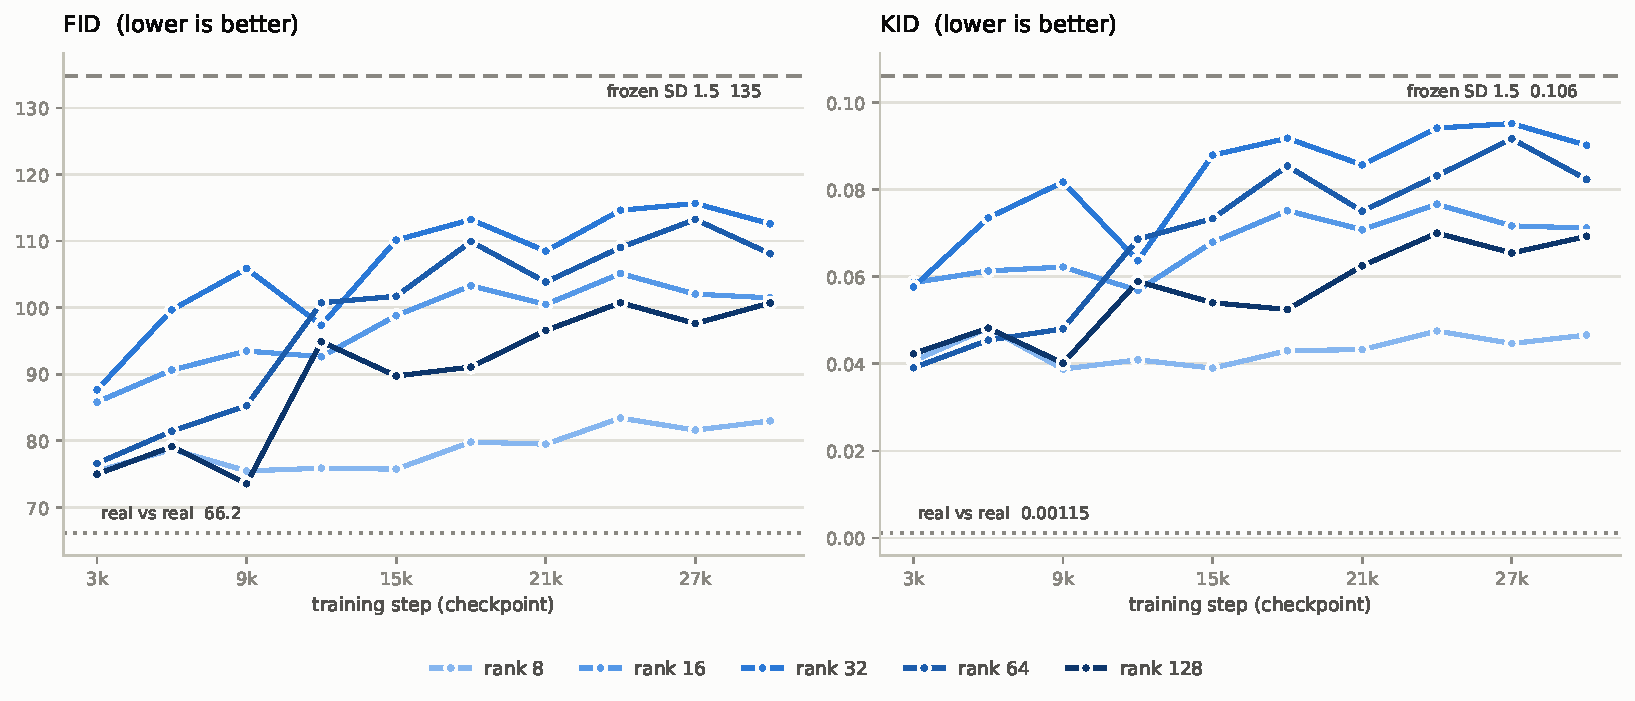
\includegraphics[width=\textwidth]{sweep.pdf}
\caption{FID and KID against training checkpoint, one line per rank
($n=500$ identical prompts and seeds per point). Dashed line: frozen SD~1.5.
Dotted line: real-vs-real noise floor.}
\end{figure}

\section*{8\quad Results}

\begin{table}[h]\centering\small
\begin{tabular}{lrrrr}
\toprule
& \multicolumn{2}{c}{Best by FID} & \multicolumn{2}{c}{Best by KID} \\
\cmidrule(lr){2-3}\cmidrule(lr){4-5}
Rank & Checkpoint & FID & Checkpoint & KID \\
\midrule
8   & 3\,000 & 75.43 & 9\,000  & 0.0388 \\
16  & 3\,000 & 85.81 & 12\,000 & 0.0569 \\
32  & 3\,000 & 87.64 & 3\,000  & 0.0577 \\
64  & 3\,000 & 76.61 & 3\,000  & 0.0391 \\
128 & 9\,000 & \textbf{73.55} & 9\,000 & 0.0401 \\
\midrule
frozen SD 1.5 & --- & 134.83 & --- & 0.1062 \\
real vs real & --- & 66.17 & --- & 0.00115 \\
\bottomrule
\end{tabular}
\caption{Best checkpoint per rank, from the 50-cell sweep.}
\end{table}

\textbf{Three findings.}

\begin{enumerate}
\item \textbf{LoRA adaptation works, and strongly.} KID falls from 0.1062
(frozen) to $\approx$0.039--0.058, a 2--3$\times$ improvement. FID falls from
134.8 to $\approx$73--88 against a floor of 66.2 --- i.e.\ the best adapted
models close most of the gap to real images.

\item \textbf{The optimum is early; 31\,000 steps is far too many.} Every rank
peaks at checkpoint 3\,000 or 9\,000 and degrades monotonically thereafter.
Training ran $\approx$10 epochs when $\approx$1--3 would have sufficed. This is
visible in the images: at step 3\,000 the Mercedes hood ornament (present in
every real Cityscapes frame, since the dataset was captured from a Mercedes) is
rendered sharply; by step 30\,000 it degenerates into a cyan blob, with magenta
patches on road surfaces. Degradation is worse at higher rank, consistent with
\texttt{lora\_alpha}$=$rank (scale $\alpha/r = 1$) meaning the same peak LR
produces larger effective updates as rank grows. Note the cosine decay puts the
last $\approx$6\,000 steps below $2\times10^{-6}$, so the degradation accumulates
during the high-LR middle of the run (roughly steps 3\,000--20\,000), not at the
tail.

\item \textbf{There is no monotonic rank trend.} Ranks 8, 64 and 128 perform
similarly ($\text{FID}\approx73$--77); ranks 16 and 32 are notably worse
($\approx86$--88). Capacity is evidently not the binding constraint --- supported
independently by $\sum\|BA\|_F$, which \emph{falls} from rank 8 (867.8) to rank 32
(688.1) before rising again: doubling capacity did not produce a larger
functional change.
\end{enumerate}

\section*{9\quad Current status and next steps}

\textbf{Complete:} preprocessing; captioning; frozen baseline (24\,995);
all five adapters trained with 10 checkpoints each; the 50-cell checkpoint sweep
(25\,000 images) and its FID/KID evaluation.

\textbf{Running:} full metric suite (FID, KID, CLIP, BLIP, LPIPS) on frozen plus
all five ranks at checkpoints 3\,000 and 9\,000.

\textbf{Next:}
\begin{enumerate}
\item Fix the evaluation checkpoint (3\,000 or 9\,000) from the sweep and the
full-suite run.
\item Regenerate evaluation sets for all five ranks at that checkpoint.
At 10\,000 images per rank this is $\approx$16\,h on two A100s; at the full
24\,995, $\approx$39\,h.
\item Final comparison: real vs frozen vs five ranks on the complete suite.
\end{enumerate}

\textbf{Open questions for discussion.}
\begin{itemize}
\item \emph{Peak learning rate not scaled with rank.} All ranks share the same
cosine schedule peaking at $2\times10^{-4}$, and \texttt{lora\_alpha}$=$rank
makes the LoRA scale factor $\alpha/r = 1$ everywhere. A rank-128 adapter
therefore has $16\times$ the parameters of rank-8 taking steps of the same size,
so its effective update to the UNet is larger. The rank axis thus mixes capacity
with update magnitude. Two ways to resolve it: scale the peak LR with rank
(e.g.\ $2\times10^{-4}\sqrt{8/r}$), at the cost of LR no longer being constant
across the sweep; or stop at $\approx$3\,000--6\,000 steps, where the sweep shows
every rank is at its best and before the high-LR phase does damage. The latter
keeps one more variable fixed and is cheaper.
\item \emph{Where the interesting variation lies.} Given saturation below rank
16, ranks 1, 2 and 4 would likely be more informative than rank 256.
\item \emph{Evaluation set size.} 10\,000 is the standard FID operating point and
would cut generation time by $\approx$60\% relative to 24\,995.
\item \emph{Error bars.} FID/KID are currently point estimates. KID subset
resampling would give variance, which matters because several rank differences
may not be significant at $n=500$.
\end{itemize}

\section*{Appendix: infrastructure notes}

\begin{itemize}
\item \textbf{Only \texttt{renyi} can run the main environment.} Its torch is
\texttt{2.11.0+cu130} (needs driver $\geq$580). Drivers: renyi 580.95.05~\checkmark,
erdos 560.35.05~$\times$, neumann 545.23.08~$\times$. On the wrong node the job
silently falls back to CPU. A second environment with \texttt{torch 2.4.1+cu121}
unlocks the V100 nodes.
\item \textbf{Throughput} ($768^2$, 30 steps): A100 0.44\,img/s; V100
0.07--0.09\,img/s sustained --- the A100 is $\approx$5$\times$ faster.
\item \textbf{Hardware equivalence verified.} The same seed on A100 and V100
gives the same image to within floating-point noise (mean abs.\ difference
0.4--0.9\,/\,255, versus 54\,/\,255 for two genuinely different samples), so
mixed-hardware generation does not compromise the comparison.
\item \textbf{Approximate GPU budget so far:} captioning 3.9\,h; frozen baseline
13.9\,h; training 46.6\,GPU-h; checkpoint sweep generation 16.1\,h; evaluation
1.3\,h. Total $\approx$\,82\,GPU-hours.
\end{itemize}

\end{document}
